\documentclass[pdftex,12pt,a4paper,english]{article}
\usepackage{lmodern}
\usepackage[T1]{fontenc}		%umlaute!
\usepackage[utf8x]{inputenc}
\usepackage[cm]{fullpage}
\usepackage[ngerman]{babel}
\usepackage[pdftex]{graphicx}
\usepackage{microtype,xcolor}             %x-Vorschlag
%\usepackage[percent]{overpic}   %ins Bild schreiben
%\usepackage{mwe}                %ins Bild schreiben


%\usepackage{epstopdf}
\usepackage{hyperref}
\usepackage{float}
\usepackage{subcaption}


%\sloppy			% Blocksatz 

\begin{document}



\begin{figure}[H]
  \begin{subfigure}[b]{.3\textwidth}
    \centering
    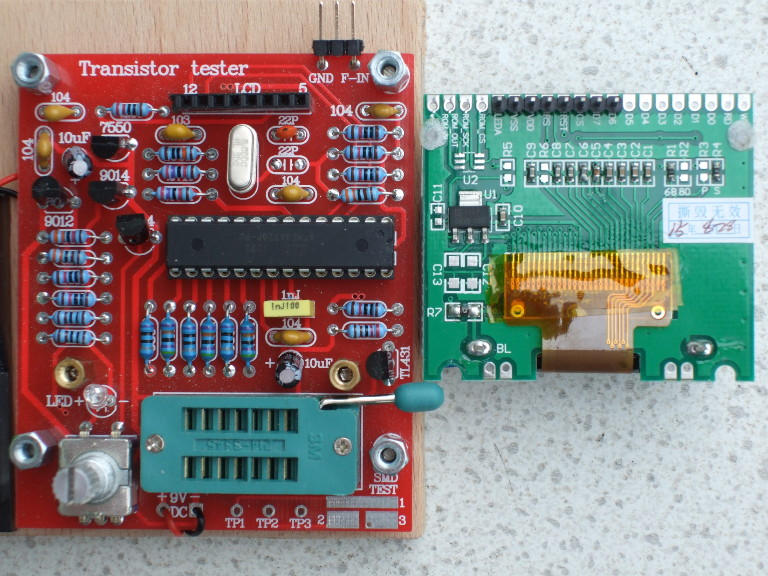
\includegraphics[width=1.\textwidth]{../PNG/Kit_ST7565b.jpg}
	  {\href{run:./trunk/mega328_st7565_kit/.}{m328\_kit}}
  \end{subfigure}
~
  \begin{subfigure}[b]{.3\textwidth}	% 9cm
    \centering
    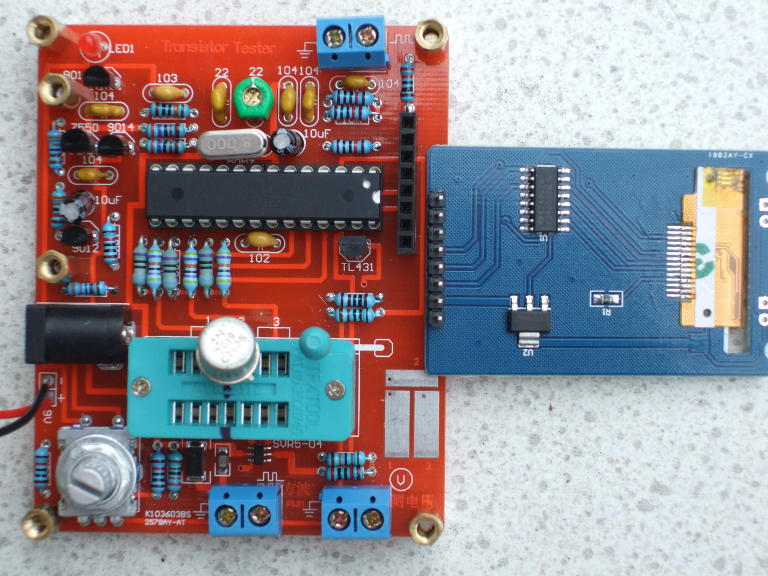
\includegraphics[width=1.\textwidth]{../PNG/Kit_Color_b.jpg}
	  {\href{run:./trunk/mega328_color_kit/.}{m328\_color\_kit}}
  \end{subfigure}
~
  \begin{subfigure}[b]{.3\textwidth}	% 9cm
    \centering
    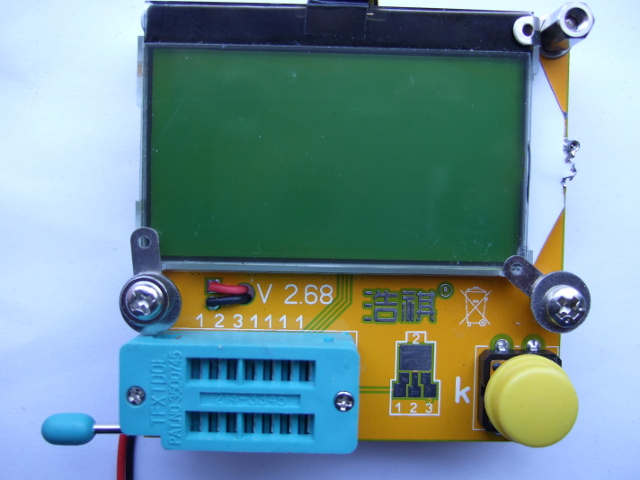
\includegraphics[width=1.\textwidth]{../PNG/T3_Front.JPG}
	  {\href{run:./trunk/mega328_T3_T4_st7565/.}{T3/T4}}
  \end{subfigure}
%  \caption{y}
\end{figure}

\begin{figure}[H]
  \begin{subfigure}[b]{.3\textwidth}
    \centering
    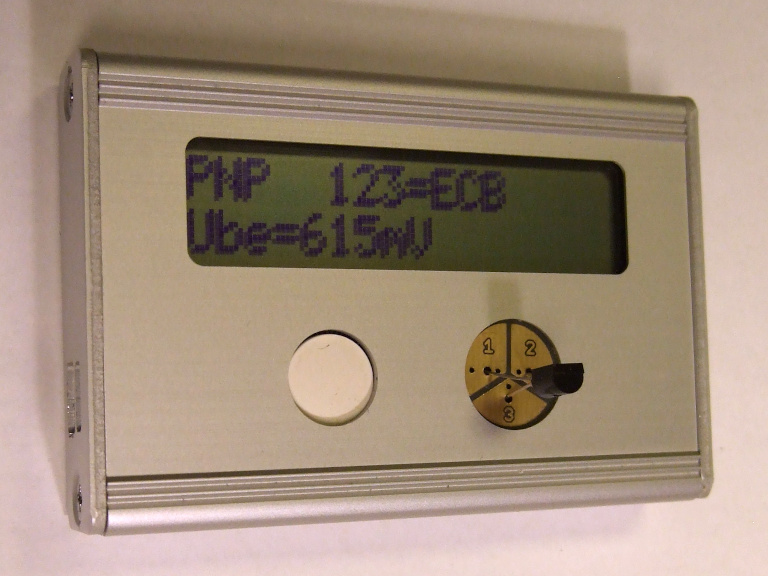
\includegraphics[width=1.\textwidth]{../PNG/Fifi_total.JPG}
	  {\href{run:./trunk/mega168_1.9V/.}{m168 1.9V}}
	  {\href{run:./trunk/mega168_3.3V/.}{m168 3.3V}} \\
	  {\href{run:./trunk/mega328_1.9V/.}{m328 1.9V}}
	  {\href{run:./trunk/mega328_3.3V/.}{m328 3.3V}}
  \end{subfigure}
~
  \begin{subfigure}[b]{.3\textwidth}	% 9cm
    \centering
    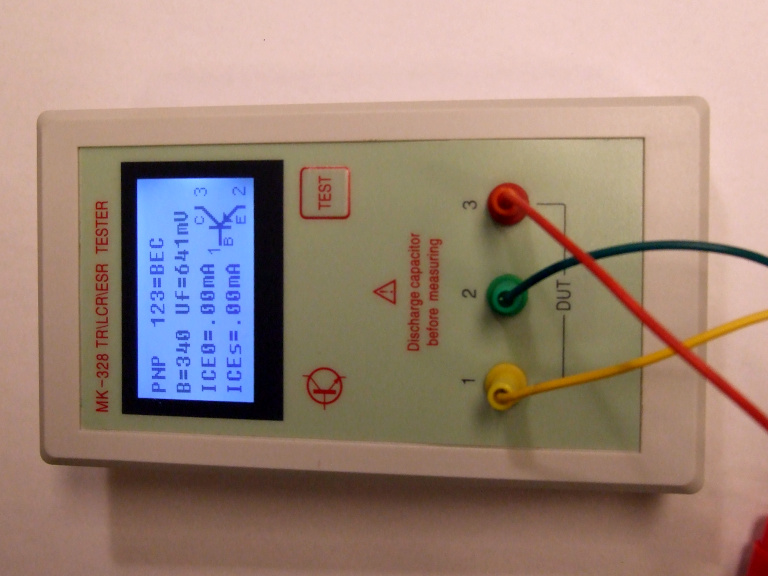
\includegraphics[width=1.\textwidth]{../PNG/MK328_total.JPG}
	  {\href{run:./trunk/mega328_MK-328/.}{m328 MK-328}}
  \end{subfigure}
~
  \begin{subfigure}[b]{.3\textwidth}	% 9cm
    \centering
    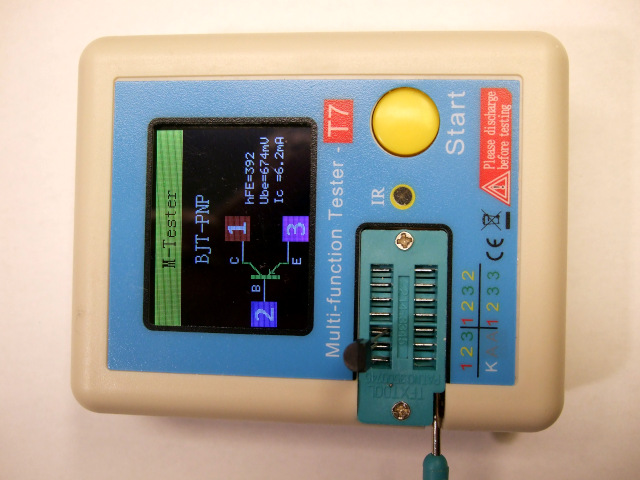
\includegraphics[width=1.\textwidth]{../PNG/T7_total.JPG}
	  {\href{run:./trunk/mega644_T7_Mod/.}{m644 T4}}
  \end{subfigure}
%  \caption{y}
\end{figure}


\end{document}

